\documentclass[11pt]{article}
\usepackage{classTools}
\usepackage{graphicx}

\begin{document}

\psHeader{3}{Wed Oct. 2, 2024 (11:59pm)}

\textbf{Your name: Emily Kang}

\textbf{Collaborators: Vennela J}

\textbf{No. of late days used on previous psets: 0}

\textbf{No. of late days used after including this pset: 0}


The purpose of this problem set is to solidify your understanding of the RAM model (and variants), and the relations between the RAM model, the Word-RAM model, Python programs, and variants. In particular, you will build skills in simulating one computational model by another and in evaluating the runtime of the simulations (both in theory and in practice).

\textit{Note: We STRONGLY recommend typing this problem set (in LaTeX, if possible) -- question 3 will probably be the longest proof we've had you write in the course so far, and unless you have typewriter handwriting, it is much easier for us to grade typed submissions. If we can't read your handwriting, chances are it will lose points.}

\begin{enumerate}
 
    \item (Simulation in practice: RAMs on Python)  
    In the Github repository, we have given you a partially written Python implementation of a universal RAM Model simulator.  Your task is to fill in the missing parts of the code to obtain a complete universal RAM simulator.
     Your simulator should take as input a RAM Program $P$ and an input $x$, and simulate the execution of $P$ on $x$, and return whatever output $P$ produces (if it halts).  The RAM Program $P$ is given as a Python list $[v,C_0,C_1,\ldots,C_{\ell-1}]$, where $v$ is the number of variables used by $P$.  For simplicity, we assume that the variables are named $0,\ldots,v-1$ (rather than having names like ``tmpptr'' and ``insertvalue''), but you can introduce constants to give names to the variables.  The $0$\textsuperscript{th} variable will always be $\inputlen$, the $1$\textsuperscript{st} variable $\outputpointer$, and the $2$\textsuperscript{nd} variable $\outputlen$.  A command $C$ is given in the form of a list of the form $[\cmd]$, $[\cmd,i]$, $[\cmd,i,j]$, or $[\cmd,i,j,k]$, where $\cmd$ is the name of the command and $i,j,k$ are the indices of the variables or line numbers used in the command.  For example,  the command $\var_i = M[\var_j]$ would be represented as $(\READ,i,j)$.  See the Github repository for the precise syntax as well as some RAM programs you can use to test your simulator.

    \item (Empirically evaluating simulation runtimes and explaining them theoretically)  

Consider the following two RAM programs:

\begin{algorithm}[H]
\Input{A single natural number $N$ (as an array of length 1)}
\Output{$13^{2^N+1}$ (as an array of length 1)}
\Variables{$\inputlen, \outputpointer, \outputlen, \counter, \result$}
\setcounter{AlgoLine}{-1}
$\zero = 0$\;
$\one = 1$\;
$\thirteen = 13$\;
$\outputlen = 1$\;
$\outputpointer = 0$\;
$\result = 13$\;
$\counter = M[\zero]$\;
\Indp
 IF $\counter == 0$ GOTO \ref{line:done}\; \label{line:loop}
$\result = \result \times \result$\;
$\counter = \counter - \one$\;
IF $\zero == 0$ GOTO \ref{line:loop}\;
\Indm
$\result = \result \times $\thirteen\; \label{line:done}
$M[\outputpointer]=\result$\;
\end{algorithm}

\begin{algorithm}[H]
\Input{A single natural number $N$ (as an array of length 1)}
\Output{$13^{2^N+1} \bmod 2^{32}$ (as an array of length 1)}
\Variables{$\inputlen, \outputpointer, \outputlen, \counter, \result, \temp, \W$}
\setcounter{AlgoLine}{-1}
$\zero = 0$\;
$\one = 1$\;
$\thirteen = 13$\;
$\outputlen = 1$\;
$\outputpointer = 0$\;
$\result = 13$\;
$\W = 2^{32}$\;
$\counter = M[\zero]$\;
\Indp
IF $\counter == 0$ GOTO \ref{line:done2}\; \label{line:loop2}
$\result = \result \times \result$\;
$\temp = \result / \W$\;
$\temp = \temp \times \W$\;
$\result = \result - \temp$\;
$\counter = \counter - \one$\;
IF $\zero == 0$ GOTO \ref{line:loop2}\;
\Indm
$\result = \result \times \thirteen$\;
\label{line:done2}
$\temp = \result / \W$\;
$\temp = \temp \times \W$\;
$\result = \result - \temp$\;
$M[\outputpointer]=\result$\; 
\end{algorithm}

\begin{enumerate}
    \item Exactly calculate (without asymptotic notation) the RAM-model running times of the above algorithms as a function of $N$.
    Which one is faster? \label{itm:RAMtime} \\
    \textit{Solution.} For the first program,
    \begin{enumerate}
        \item Lines $0$ through $6$ run once.
        \item Lines $7$ through $10$ run $N$ times.
        \item Line $7$ runs one more time when $\counter$ is $0$.
        \item Lines $11$ and $12$ run once.
    \end{enumerate}
    Therefore the final runtime is $7+(4N+1)+1+1 = \boxed{4N+10}$.

    For the second program,
    \begin{enumerate}
        \item Lines $0$ through $7$ run once.
        \item Lines $8$ through $14$ run $N$ times.
        \item Line $8$ runs one more time when $\counter$ is $0$.
        \item Lines $15$ and $19$ run once.
    \end{enumerate}
    Therefore the final runtime is $8+(7N+1)+5 = \boxed{7N+14}$. \\
    We see that the \boxed{\text{first program}} has faster runtime.
    \item Using your RAM Simulator, run both RAM programs on inputs $N=0,1,2,\ldots,15$ and graph the actual running times (in clock time, not RAM steps).  (We have provided you with some timing and graphing code in the Github repository.) Which one is faster?  \label{itm:realtime}  
    \textit{Solution.}
    \begin{figure}[H]
        \centering
        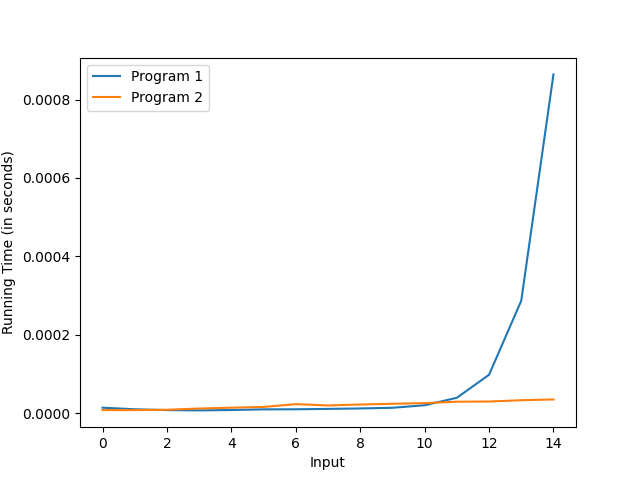
\includegraphics[width=0.5\textwidth]{Figure_1.png}
        \caption{Graph of Running Times}
        \label{fig:example}
    \end{figure}
    As we can see, for larger imputs, the \boxed{\text{second program}} performs better than the first. While the first program performs slightly better for small inputs, for larger inputs, the first program's runtime seems to increase exponentially, whereas the second program the runtime seems to only slightly increase even for large inputs.
   
    \item Explain the discrepancies you see between Parts~\ref{itm:RAMtime} and \ref{itm:realtime}.  (Hint: What do we know about the relationship between the RAM and Word-RAM models, and why is it relevant to how efficiently the Python simulation runs?) \\
    \textit{Solution.} In part~\ref{itm:RAMtime}, we saw that theoreticaly the first program has faster runtime, but in actuality, in part\ref{itm:realtime} the second program ended up performing better for large inputs. To explain this discrepancy, we see that for larger inputs, the first program is running multiplication without bounding the numbers. This can lead to multiplication with arbitrarily high numbers which can take a long time to compute in reality, as Python will have to spend time converting the numbers to their BigNum representation. However, within the second program, we bound the results and other numbers that could get very high in value by $2^{32}$ using $mod$. Concretely, $\result$ is always bounded by $2^{32}$, so we never end up performing multiplication with extensively high numbers in the second program. As we said previously, in the first program, this could occur for large inputs, which is when we start to see a large slowdown compared to the second program. When we found runtime theoretically we assumed that these operations took constant time no matter the size of the input, which resulted in this discrepancy.
    
    \item (optional\footnote{This problem won't make a difference between N, L, R-, and R grades.}) Give a theoretical explanation of the shapes of the runtime curves you see in Part~\ref{itm:realtime}, by providing explicit formulas for the asymptotic runtimes of the two programs (in clock time). You may need to do some research online and/or make guesses about how Python operations are implemented to come up with your estimates. \\
    \textit{Solution.} To analyze the runtime behavior of both programs in Part 2b, we need to consider the effects of Python's handling of large numbers.

    Program 1 calculates $13^{2^N + 1}$, with a theoretical initial runtime of $O(N)$ due to an iteration loop. However, as $N$ increases, the number size grows exponentially, requiring Python to switch to bignum arithmetic. This switch leads to increased runtime complexity due to the Karatsuba multiplication algorithm, which is used for large integers and has a complexity of $O(d \cdot \log(d))$, where $d$ is the number of digits. Consequently, the runtime for Program 1 becomes approximately:
    
    $$
    T_1(N) \approx O(N \cdot 2^N \cdot \log(2^N)),
    $$
    
    resulting in super-exponential growth once $N$ exceeds a certain threshold.
    
    Program 2 calculates $13^{2^N + 1} \mod 2^{32}$, which keeps all calculations within the 32-bit limit, allowing Python to use constant-time integer arithmetic. Thus, the runtime for Program 2 is:
    
    $$
    T_2(N) = O(N),
    $$
    
    exhibiting consistent linear growth as each iteration is performed in $O(1)$ time.
    
    For small $N$, both programs have similar runtimes. As $N$ increases, Program 1's runtime escalates sharply due to the transition to bignum arithmetic and the complexity of large-number operations, typically around $N \approx 6$ or $7$. In contrast, Program 2 maintains a linear growth rate, highlighting the impact of keeping calculations within fixed-size integer limits.
    
    The divergent runtime curves illustrate the significance of Python's integer handling and the efficiency benefits of restricting operations to manageable integer sizes, particularly highlighting the influence of algorithms like Karatsuba in managing large numbers.
    
\end{enumerate}

\item (Simulating Word-RAM by RAM) For every Word-RAM program $P$, there is a RAM program $P'$ that simulates $P$ in the sense that:
\begin{enumerate}
    \item $P'$ halts on $(w,x)$ iff $P[w]$ halts on $x$, and 
    \item If $P[w]$ crashes, then $P'$ halts with $\outputpointer=\outputlen=0$. (We are using this output setting to indicate \crash, since the RAM model does not have any crashing in its semantics.)
    \item If $P[w](x)$ halts without crashing, then the output of $P'(x,w)$ equals the output of $P[w](x)$.
     Furthermore,   
       $$\Time_{P'}(x) = O\left(\Time_{P[w]}(x)+n+w\right),$$
where $n$ is the length of $x$.

(This was stated without proof in Lecture Notes 8.) 

\end{enumerate}

Your proof should use an {\em implementation-level} description, similar to the proof that RAM programs can be simulated by ones with at most $c$ registers in Lecture 7.  Recall that Word-RAM programs have a finite but changing memory size $S$ and a read-only variable $\wordlen$; you may want to start your simulation by calculating $S$ and $2^{\wordlen}$.  Then think about how each operation of a Word-RAM program $P$ can be simulated in a RAM program $P'$, taking care of any differences between their semantics in the Word-RAM model vs. the RAM model. Don't forget MALLOC!

\textit{Solution. }For every Word-RAM program $P$, we will prove there is a RAM program $P'$ that simulates $P$ following conditions (a), (b), and (c). Let us define a valid $P'$.
\begin{enumerate}
    \item \textbf{Crashing: } 
    \begin{enumerate}
        \item On a crash, we set \texttt{output\_ptr = 0} and \texttt{output\_len = 0}, then halt by calling \texttt{return}. This results in an empty output, indicating a crash. The process runs in constant time due to only involving two assignments.
    \end{enumerate}
    \item \textbf{Initialization: } 
    \begin{enumerate}
        \item In $P'$, we can set a variable \texttt{size} $= 2^w$, where $w$ is the word length parameter provided to $P'$. This simulates the \texttt{size} variable in Word-RAM programs that sets an upper bound for any constant or input for the program. To set \texttt{size} $= 2^w$, we can use a bitwise left shift operation, which takes constant time. All other operations to initialize \texttt{size} take constant time.
        \item Usually, in the standard RAM model, to initialize, the input $x$ of size $n$ has each of the $n$ input values placed into memory at $M[0], \ldots, M[n-1]$. In $P'$, we also check if each $M[i] \geq \texttt{size}$, after which $P'$ will crash. This takes $O(n)$ time.
        \item In $P'$, we will also set a variable \texttt{S} that keeps track of the current size of the memory array $M$. As $M$ currently contains only the input $x$ of size $n$, we initialize \texttt{S} $= n$. This takes constant time.
    \end{enumerate}
    From the above, we know that overall initialization takes $O(n + w)$ time.
    \item \textbf{GOTO: } The \texttt{goto} command will not invoke a crash; therefore, it remains the same in $P'$ as in $P$.
    \item \textbf{Arithmetic: } In Word-RAM, when we have a value greater than $\texttt{size} - 1 = 2^w - 1$ or less than $0$, we must bound the result between $0$ and $\texttt{size} - 1$. Therefore, we can simulate each arithmetic operation from $P$ into $P'$ as follows:
    \begin{enumerate}
        \item $\text{result} = a + b$ becomes $\text{result} = \min(a + b, \texttt{size} - 1)$
        \item $\text{result} = a - b$ becomes $\text{result} = \max(a - b, 0)$
        \item $\text{result} = a \times b$ becomes $\text{result} = \min(a \times b, \texttt{size} - 1)$
        \item $\text{result} = a // b$ remains the same in $P'$ as in $P$ (both models already only have nonnegative integers and integer division)
    \end{enumerate}
    We have constructed $P'$ such that no variable will be out of bounds, as $\texttt{result}$ is never greater than or equal to $\texttt{size}$ or less than zero. If it is, we crash. Note that we are only adding a constant number of operations.
    \item \textbf{Assignment: } 
    \begin{enumerate}  
        \item When assigning a constant to a variable in $P'$, we must first check whether the constant is greater than or equal to \texttt{size}. If so, we crash. Otherwise, $P'$ is implemented the same as $P$.
        \item When assigning a random function called on a variable to a variable in $P'$, $P'$ is implemented the same as $P$.
        \item When assigning a random function called on a constant to a variable in $P'$, we must first check whether the constant is greater than or equal to \texttt{size}. If so, we crash. Otherwise, $P'$ is implemented the same as $P$.
    \end{enumerate}
    Again, we have constructed the variable assignment in $P'$ such that no variable will be out of bounds, as $\texttt{result}$ is never greater than or equal to $\texttt{size}$ or less than zero. If it is, we crash. Note that we are only adding a constant number of operations.
    \item \textbf{Memory: } Word-RAM supports \texttt{malloc}, \texttt{reads}, and \texttt{writes}. For $P'$:
    \begin{enumerate}
        \item \texttt{malloc(k)}: When \texttt{malloc(k)} is called with $k$, we first check if $S + k > \texttt{size}$. If so, we crash. Otherwise, we set $S = S + k$ while $S$ remains within our set bounds.
        \item \texttt{Read} ($\texttt{var} = M[i]$): If $i < S$, $P'$ is the same as $P$. Otherwise, the operation is skipped.
        \item \texttt{Write} ($M[i] = \texttt{var}$): If $i < S$, $P'$ is the same as $P$. Otherwise, the operation is skipped.
    \end{enumerate}
    Note that we are only adding a constant number of operations.
    \item \textbf{Return: } For $P'$, we have $M[\texttt{output\_ptr}], \dots, M[\min(\texttt{output\_ptr} + \texttt{output\_len} - 1, S - 1)]$, which ensures that when returning the output, we do not try to access indices greater than or equal to $S$, our current amount of allocated memory. Note that we are only adding a constant number of operations.
\end{enumerate}

We have now completed the design of $P'$, allowing us to verify that the three required statements hold under our design.

To verify (a), we consider that halting in $P'$ can occur with or without a crash. $P'$ is defined to crash only if constants or input values $x[i]$ (for $i \in \{0, \dots, n-1\}$) are greater than or equal to $2^w$, or if $S$ is set to a value larger than $2^w$—either initially or through \texttt{malloc}. These conditions align with those under which a Word-RAM model would crash, meaning $P'$ crashes if and only if $P(x)$ crashes. Since we translated each operation from $P(x)$ to $P'$ to maintain identical behavior, the programs will behave the same in every scenario. Therefore, whenever $P(x)$ halts, so does $P'$, and vice versa.

To verify (b), we confirm that $P'$ correctly handles crashes. In $P'$, if a crash occurs, we set $\texttt{output\_ptr} = 0$ and $\texttt{output\_len} = 0$, and then halt by returning immediately. Since these actions consistently occur whenever there is a crash, and since the program halts after setting these values, statement B holds true.

To verify (c), we analyze the runtime of $P'$, denoted as $T_{P'}(x)$. This time includes both the initialization time and the command execution time:

\[
T_{P'}(x) = T_{\text{Initialization}} + T_{\text{All other operations}}
\]

We previously showed that $T_{\text{Initialization}} = O(n + w)$. Since the operations in $P'$ introduce only a fixed number of constant-time operations, the asymptotic running time is not increased compared to the original RAM model. Thus, the execution time of the remaining commands is the same as in $P(x)$, meaning $T_{\text{All other operations}}(x) = T_{P}(x)$. Therefore, the total time complexity of $P'$ is:

\[
T_{P'}(x) = O(n + w) + T_{P}(x) = O(T_{P}(x) + n + w)
\]

We have successfully designed $P'$ to simulate $P$ and proved that all three points in the problem statement hold true.


\item (reflection) Discuss the value (or lack thereof) that you think computational models, and the RAM and Word-RAM models in particular, have for computer science.  All opinions are valid, as long as they show serious thought and are backed by specific justifications.

\textit{Note: As with the previous psets, you may include your answer in your PDF submission, but the answer should ultimately go into a separate Gradescope submission form.}

\item Once you're done with this problem set, please fill out \href{https://forms.gle/TG8cG4LWN3S4T6za6}{this survey} so that we can gather students' thoughts on the problem set, and the class in general. It's not required, but we really appreciate all responses!

\end{enumerate}


\end{document}
